%!TEX root = ../../Heun_Dale_Haney_A_dynamic_approach_to_input_output_modeling.tex
%%%%%%%%%%%%%%%%%%%%% chapter.tex %%%%%%%%%%%%%%%%%%%%%%%%%%%%%%%%%
%
% sample chapter
%
% Use this file as a template for your own input.
%
%%%%%%%%%%%%%%%%%%%%%%%% Springer-Verlag %%%%%%%%%%%%%%%%%%%%%%%%%%
%\motto{Use the template \emph{chapter.tex} to style the various elements of your chapter content.}
\chapter{Material flows}
% use \chaptermark{}
% to alter or adjust the chapter heading in the running head
\chaptermark{Materials}
% Always give a unique label
\label{chap:materials} 

\abstract*{[NEED TO ADD ABSTRACT HERE]}

%% \abstract{Each chapter should be preceded by an abstract (10--15 lines long) that summarizes the content. The abstract will appear \textit{online} at \url{www.SpringerLink.com} and be available with unrestricted access. This allows unregistered users to read the abstract as a teaser for the complete chapter. As a general rule the abstracts will not appear in the printed version of your book unless it is the style of your particular book or that of the series to which your book belongs.\newline\indent
%% Please use the 'starred' version of the new Springer \texttt{abstract} command for typesetting the text of the online abstracts (cf. source file of this chapter template \texttt{abstract}) and include them with the source files of your manuscript. Use the plain \texttt{abstract} command if the abstract is also to appear in the printed version of the book.}

%% Use the template \emph{chapter.tex} together with the Springer document class SVMono (monograph-type books) or SVMult (edited books) to style the various elements of your chapter content in the Springer layout.

In the Introduction, we introduced the idea that economies are
in many ways like organisms. The job of this chapter is to explore
this idea further by observing the interchange of materials \emph{within}
an economy, as well as exchanges of materials between an economy and 
surrounding environment---the biosphere.

There are many easily observable instances of material flow within an
economy. I look around my office at my computer screen and coffee cup
and myriad other items. I look out my window to the street and building
opposite. All of these goods came originally from natural resources, be it paper or
petroleum or rock. They were extracted and processed, transported and
transformed requiring yet more materials and energy inputs in the form of
electricity or fuels. 

There are also inumerable material flows caused by an economy that we do not observe.
The extraction of raw materials generates additional overburden---earth that must be
extracted and processed and ultimately discarded without ever entering the economy
proper. Other flows occur around us unseen. The cars outside my window suck in nitrogen
and oxygen (without which the engine would not work) and emit water, carbon dioxide and
other more harmful substances. 

Even services which we tend to think of as non-material, require at least some material
infrastructure. The hairdresser requires scissors (and to a greater or lesser extent 
some hair) with which to work. Even the internet, often lauded as the exemplar of
dematerialization of the economic process, requires a whole host of computer
infrastructure including electricity, data servers, telephone networks and a
computer by which to access it.

In this chapter, we will define a mathematical framework by which to track the flow of
materials within an economy, building from a one-sector economy up to examples of both a
two- and three-sector economy. We will finally apply this framework to the illustrative
example of the US automobile industry that runs through the whole book. First let us
outline the basic methodology.

\section{Methodology}

% Everyone is familiar with the notion of accounting of material (and even non-material)
% things. In order to be rigorous, the first step requires the definition of what we
% will be counting as well as the place (defined in both time and space) for which we will
% be counting. Engineers often call this a \emph{control volume}. For example, I may wish
% to account the number of apples in my home over a week-long period. In which case,
% I would count the number of apples that enter  and leave my home, as well as any apples
% that are eaten and, just in case I happen to have an apple tree, any apples that grow
% inside my home. Our accounting equation would look something like:

This book is about counting both money and energy:
both are important for the world in which we live.
An entire academic discipline and industry is focused on counting money (accounting).
Energy is an extremely important resource for the economies of the world, 
And, we believe that money and energy interplay 
in ways that shaped the past and will influence the future.
In this section, we define rigorous ``counting'' methods that will be applied
to money and energy throughout this book.

Everyone counts material (and even non-material) things. 
Rigorous counting requires precise definition of both 
what we will be counting
and the place (defined in both time and space) for which we will be counting. 
Engineers often call this definition a \emph{control volume}. 
For example, I may wish to count (or make an accounting of, or simply ``account'') 
the number of apples in my home over a week-long period. 
To do so, I would count the number of apples that enter and leave my home, 
any apples that are eaten (consumed),
and, in the event that I happen to have an apple tree, 
any apples that I grow (produce). 
A rigorous accounting equation for my apples would be:

\begin{equation}
	\Delta\textrm{apples} = \textrm{apples in} - \textrm{apples out} + \textrm{apples grown} - \textrm{apples eaten}
\end{equation}

\noindent More generally, we may say:

\begin{equation}
	\textrm{Accumulation}
	= \textrm{Transfers in} 
	- \textrm{Transfers out}
	+ \textrm{Production}
	- \textrm{Consumption}
\end{equation}

Rather than looking at the total amount of apples over our week-long period, 
we may consider the flow of apples ($A$), per unit time, e.g. apples per day, 
in which case our accounting equation would look like:

\begin{equation}
	\frac{\mathrm{d}A}{\mathrm{d}t}
	= \dot{A}_{in}
	- \dot{A}_{out}
	+ \dot{A}_{grown}
	- \dot{A}_{eaten}
\end{equation}

\noindent where the dot above the variable indicates the flow rate per unit time and
$\frac{\mathrm{d}}{\mathrm{d}t}$ is the rate of change of the quantity
being counted, or the accumulation rate.

In the discussion that follows, we will be making great use of the First Law of 
Thermodynamics, which is a fancy way of saying that, when we discuss \emph{mass}, i.e.
materials, and \emph{energy}, the First Law tells us that these entities can neither be
created or destroyed. In other words, the last two terms of our accounting equation
will always be equal to zero. We also distinguish between four different types of
materials flowing into or out of a production sector: products ($\dot{P}$), resources ($\dot{R}$),
short-lived goods ($\dot{S}$) and capital goods ($\dot{K}$), as shown in Figure
\ref{fig:PERKS_materials}. 

Resource materials ($\dot{R}$) always enter the sector on the left and comprise those materials that
are destined to end up \emph{embodied} in the goods produced by the sector ($\dot{P}$), except
for some proportion that are wasted and leave from the bottom of the sector and are
returned to the biosphere. For example, sheet metal, rubber and glass (as well as
many, many other materials) enter the automobile sector as resources and end up as part
of the cars that are produced. Some fraction of these materials may not make it into the
final product, such as trimming scrap from metal parts stamping, and may be either
recycled internally, or sent to scrap. Resource materials are not be accumulated within
a sector.

Short-lived goods ($\dot{S}$) include those materials that are necessary for the production
processes of a sector, but are neither accumulated within the sector, nor make it into
the products themselves. They enter the sector from above and leave the sector from
below and return to the biosphere. Examples of these short-lived flows include 
energy resources needed to run the sector, including the contribution from labor, and
any water used in processing. A number of material flows, such as production equipment,
are necessary for the continued operation of a sector but are not counted as short-lived
goods, since the processes are dependent upon the accumulation of these materials within
the sector. Such flows are instead counted as capital goods ($\dot{K}$). These flows also enter from
above, but are stored within the sector (represented by storage tanks) and leave the
sector as capital depreciation from below to be returned to the biosphere. 


All products ($\dot{P}$) leave the sector from the right. Some of this flow is returned to the 
sector as self-consumption of either resources ($\dot{R}$), short-lived ($\dot{S}$) or capital goods ($\dot{K}$), the rest
flows either to be used by other sectors within the economy, or flows to final demand. 


\begin{figure}[h!]
\centering
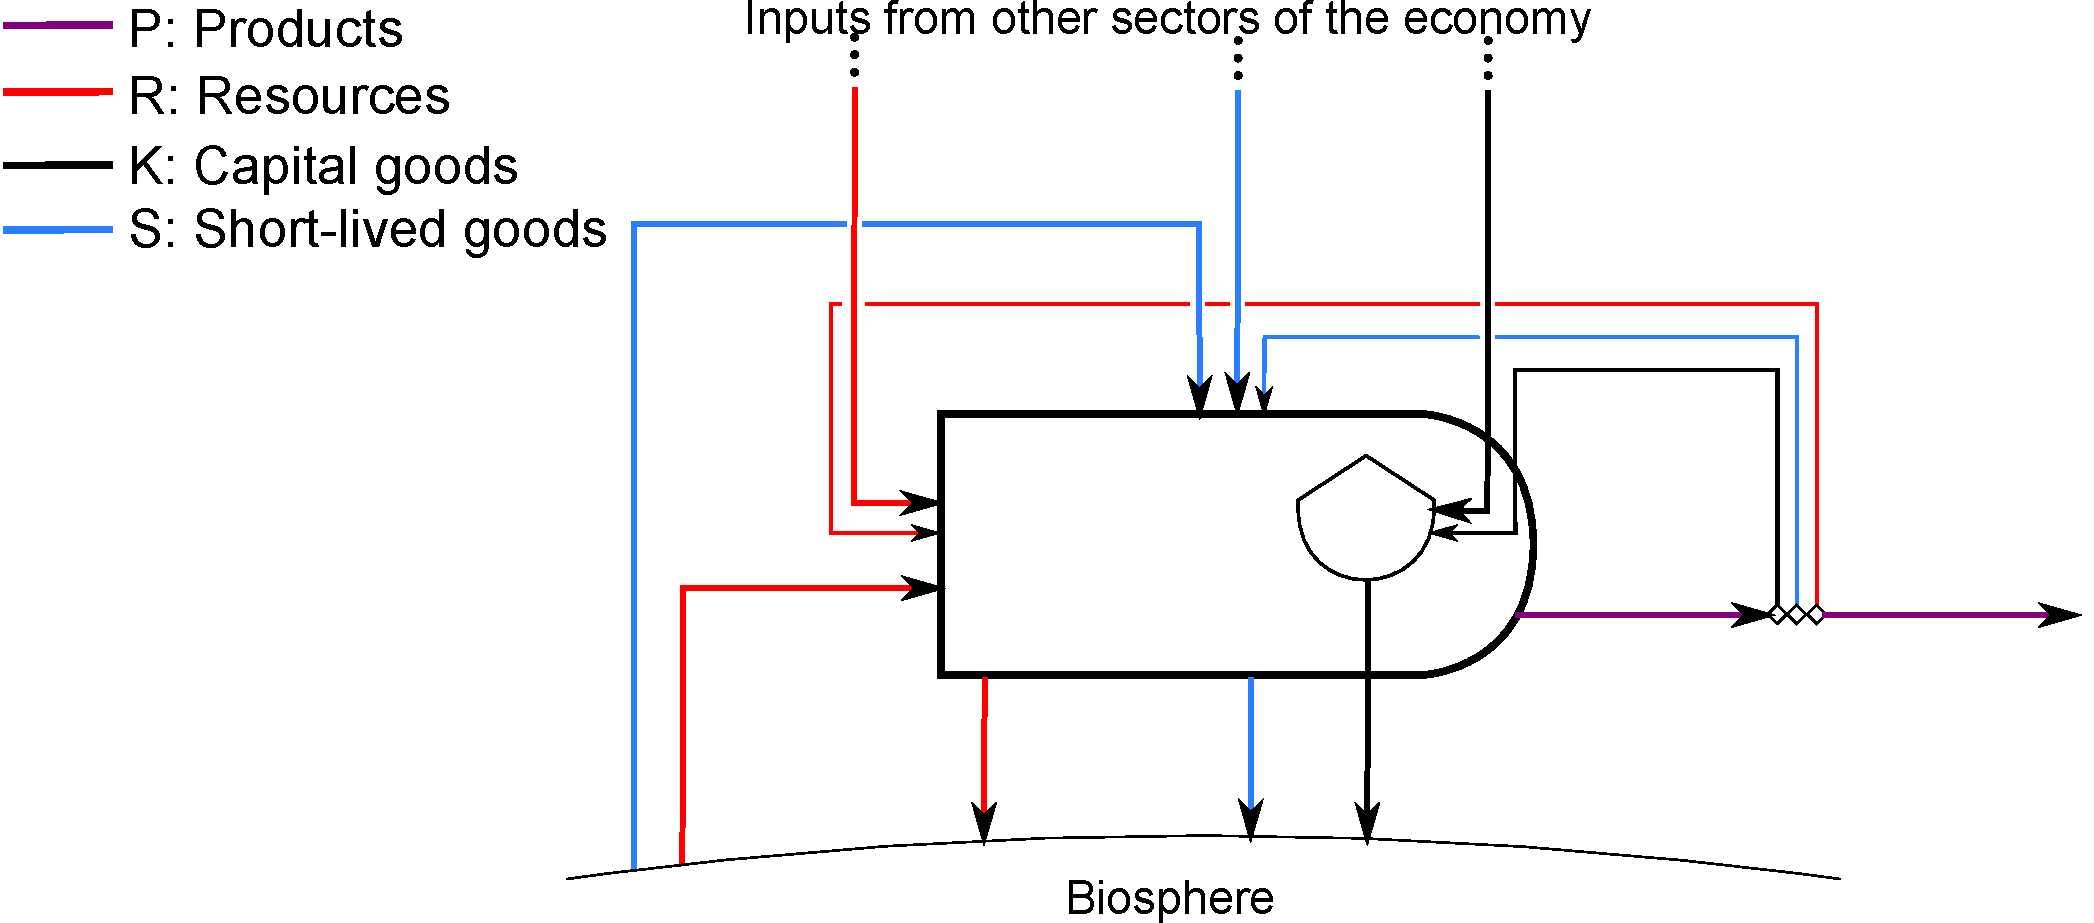
\includegraphics[width=0.8\linewidth]{Part_1/Chapter_Materials/images/PERKS_basic_unit_materials.pdf}
\caption{Material flows into and out of a single sector of the economy. Resource flows ($\dot{R}$) enter the sector from the right and are embodied in products ($\dot{P}$) which leave from the left. Some waste resources are leave the sector at the bottom and are returned to the biosphere. Short-lived material flows ($\dot{S}$) enter the sector from above and leave from below to return to the biosphere.  Only capital flows ($\dot{K}$) may accumulate within the sector, depicted by the storage tank. These also enter the sector from above. Depreciated capital leaves the sector from below and is returned to the biosphere.}
\label{fig:PERKS_materials}
\end{figure}

%%%%%%%%%% Materials: Example A %%%%%%%%%%
\section{Example A: one sector economy}
\label{sec:A_materials}
%%%%%%%%%%


Our first example looks at the case where all processes within the economy occur within
one sector, we do not distinguish between production and consumption, as depicted in
Figure \ref{fig:A_materials}. Resources ($\dot{R}$) and short-lived materials ($\dot{S}$) flow into the economy (1) from the bioshpere (2). These materials are processed within the economy into
capital goods ($\dot{K}$) which are able to be accumulated. Waste resources and used short-lived
materials are returned to the biosphere without accumulating. Capital goods are returned
to the biosphere upon depreciation.

Drawing control volumes around both the biosphere and the economy, we can consruct
our material accounting equations, such that:

\begin{align}\label{eq:A_CV_0_to_1}
	\frac{\mathrm{d}R_0}{\mathrm{d}t}		
	+	\frac{\mathrm{d}S_0}{\mathrm{d}t}
	+	\frac{\mathrm{d}K_0}{\mathrm{d}t}		&	
	=	\dot{R}_{10}		
	+	\dot{S}_{10}	
	+	\dot{K}_{10}											
	-	\dot{R}_{0}											
	-	\dot{S}_{0}								\\
	\frac{\mathrm{d}R_{1}}{\mathrm{d}t}
	+ \frac{\mathrm{d}S_{1}}{\mathrm{d}t}
	+ \frac{\mathrm{d}K_{1}}{\mathrm{d}t}		&
	= \dot{R}_{01} 
	+ \dot{S}_{01} + \dot{S}_{11}
	- \dot{S}_{1}				
	- \dot{R}_{10}				
	- \dot{S}_{10}				
	- \dot{K}_{10}											
\end{align}

\noindent Remembering that neither resources nor short-lived goods accumulate within economic sectors, tells us that:

\begin{equation}\label{eq:A-dS_1/dt_zero}
	\frac{\mathrm{d}S_1}{\mathrm{d}t}
	= \frac{\mathrm{d}R_1}{\mathrm{d}t}
	= 0.
\end{equation}

\noindent Additionally, we may also say that:

\begin{equation}\label{eq:A_S11}
	\dot{S}_{11} = \dot{S}_{1},
\end{equation}

\noindent such that our material accumulation equation \ref{eq:A_CV_0_to_1} becomes:

\begin{align}\label{eq:A_CV_0_to_1_b}
	\frac{\mathrm{d}R_0}{\mathrm{d}t}		
	+	\frac{\mathrm{d}S_0}{\mathrm{d}t}
	+	\frac{\mathrm{d}K_0}{\mathrm{d}t}		&	
	=	\dot{R}_{10}		
	+	\dot{S}_{10}	
	+	\dot{K}_{10}											
	-	\dot{R}_{0}											
	-	\dot{S}_{0}								\\
	\frac{\mathrm{d}K_{1}}{\mathrm{d}t}		&
	= \dot{R}_{01} 
	+ \dot{S}_{01} 
	- \dot{R}_{10}				
	- \dot{S}_{10}				
	- \dot{K}_{10}											
\end{align}

\begin{equation} \label{eq:A_K0_balance}
	\frac{\mathrm{d}K_{0}}{\mathrm{d}t}		
	= \dot{K}_{10}
\end{equation}

\begin{figure}[h!]
\centering
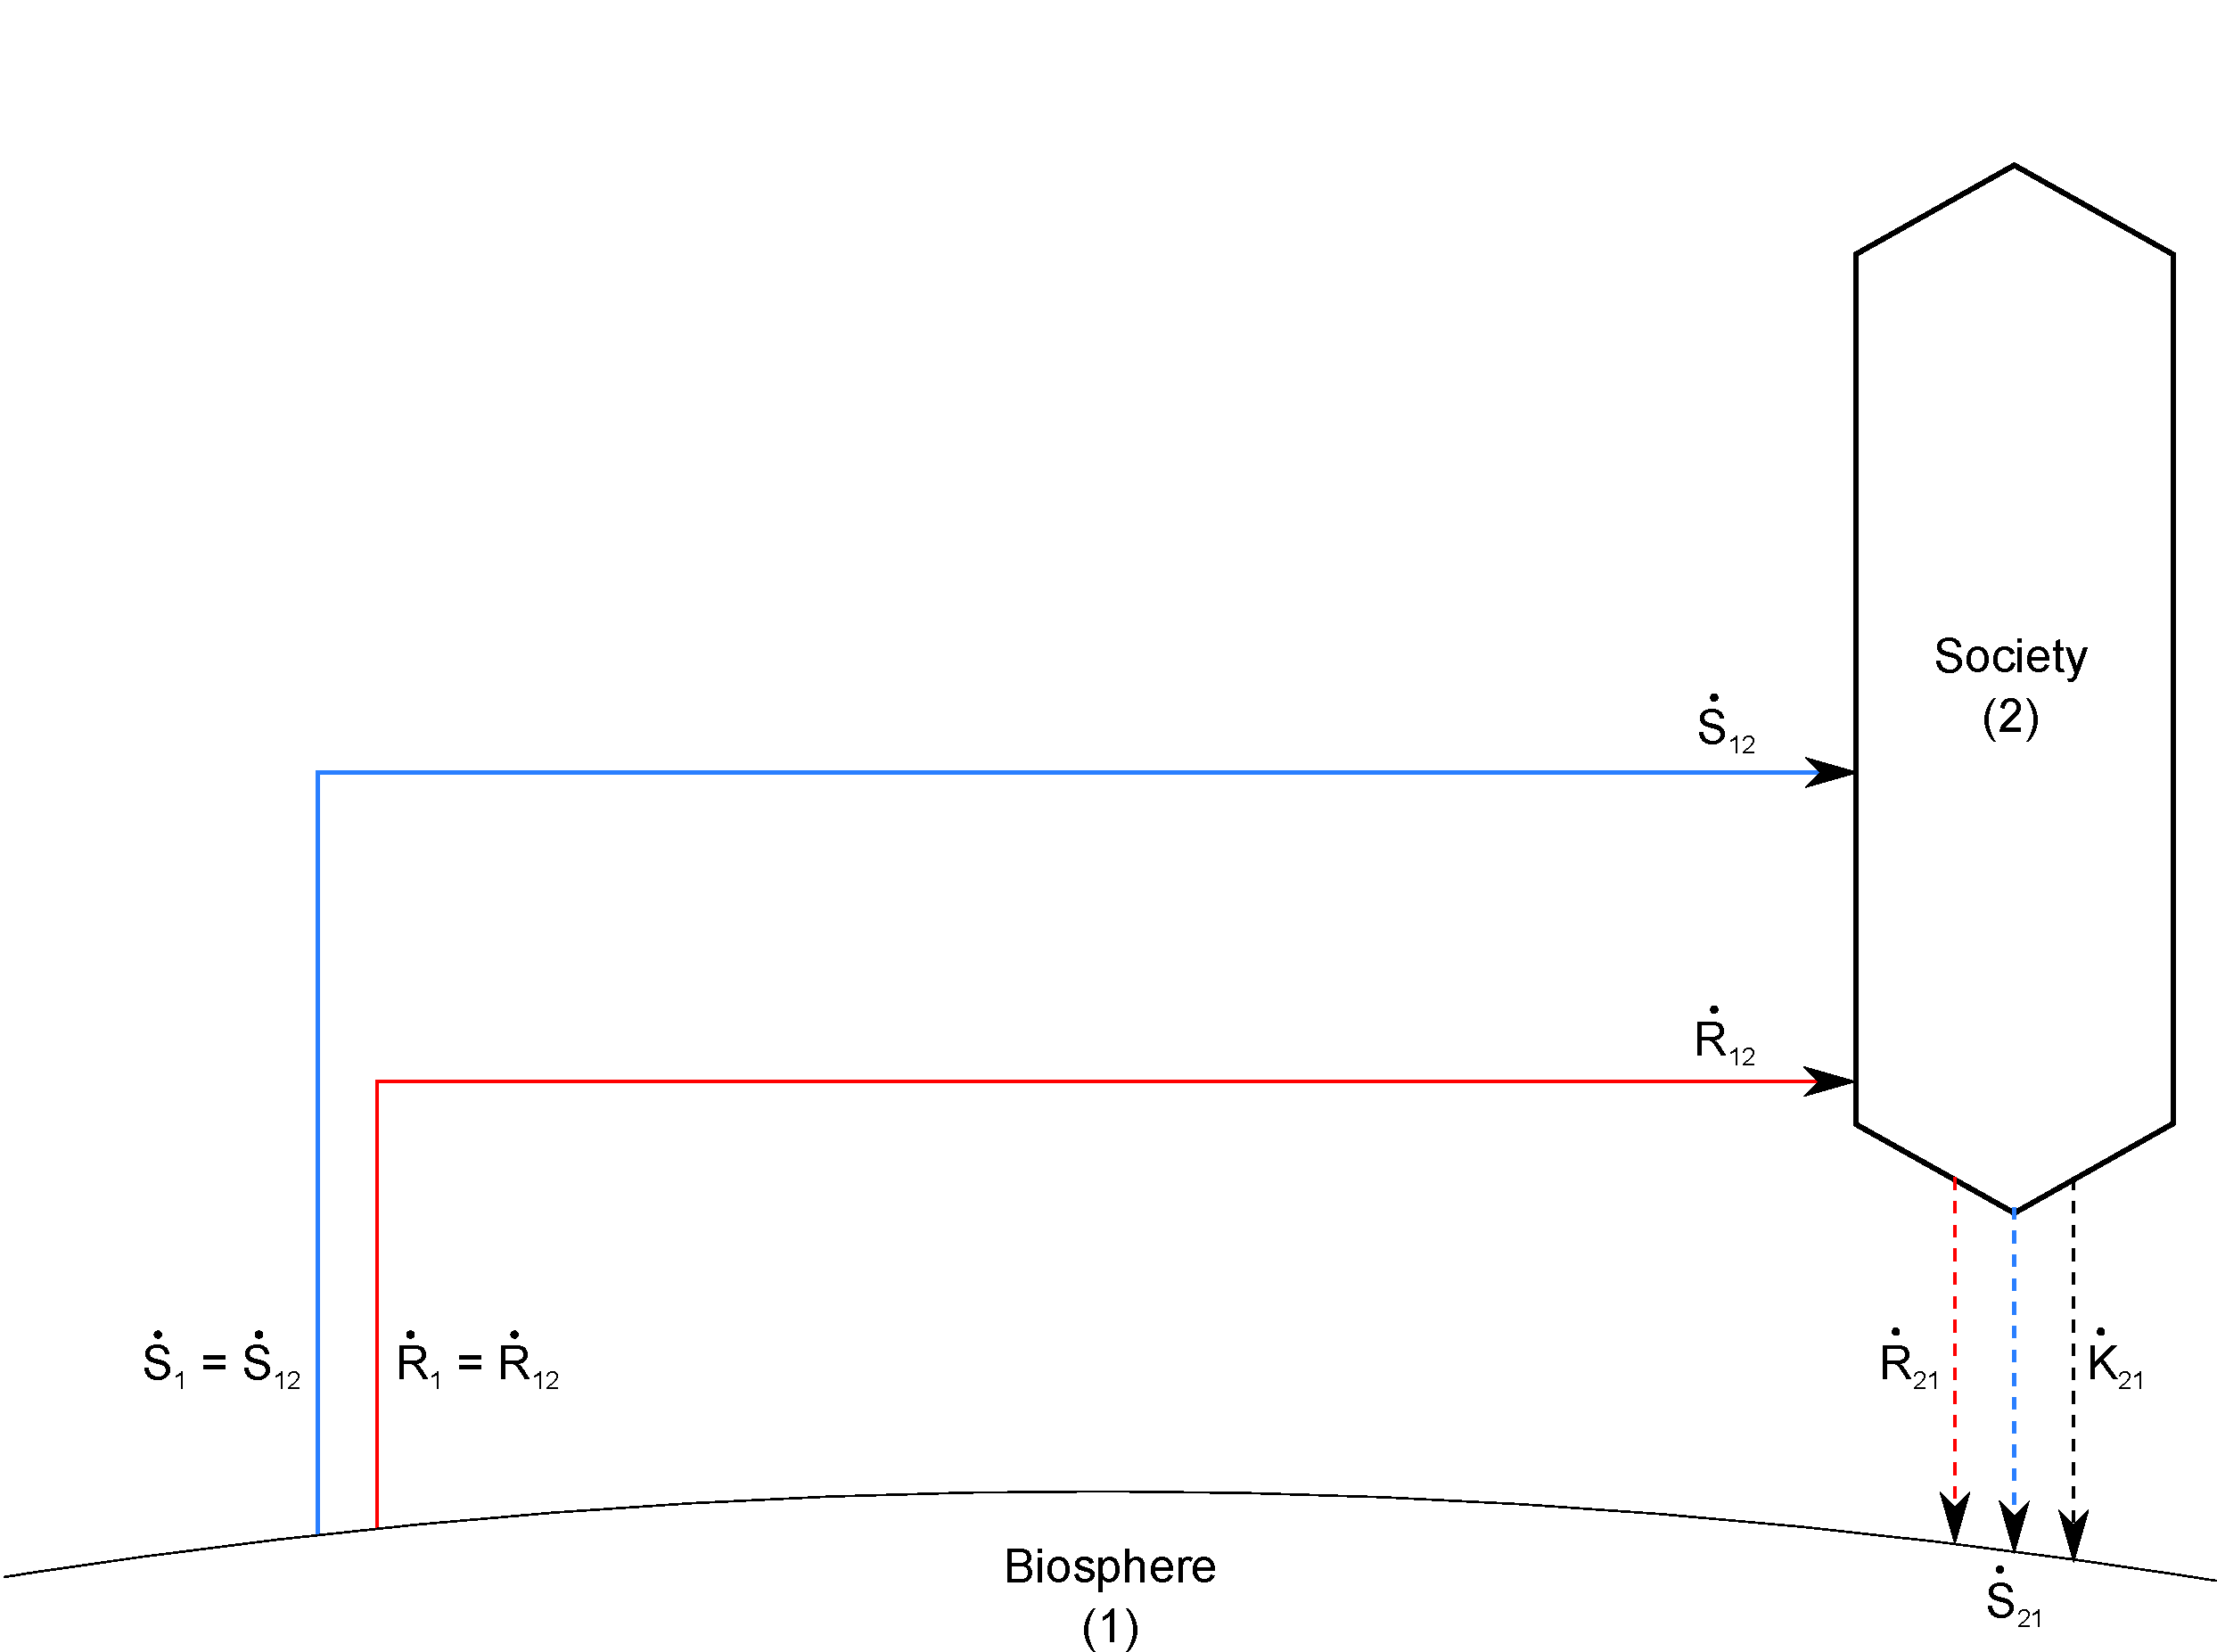
\includegraphics[width=0.8\linewidth]{Part_1/Chapter_Materials/images/1_sector_materials.pdf}
\caption{XXXX}
\label{fig:A_materials}
\end{figure}

%%%%%%%%%% Materials: Example B %%%%%%%%%%
\section{Example B: two sector economy}
\label{sec:B_materials}
%%%%%%%%%%

In our second example B, we split society into two sectors: production and consumption as depicted in Figure \ref{fig:B_materials}. Sector 2 produces goods and services for consumption in society (1). Again, setting control volumes around the biosphere and our two sectors, our accumulation equation is now written:

\begin{align} \label{eq:B_CV_0_to_2}
	\frac{\mathrm{d}R_{0}}{\mathrm{d}t} 
	+ \frac{\mathrm{d}S_{0}}{\mathrm{d}t}	
	+ \frac{\mathrm{d}K_0}{\mathrm{d}t}		&
	=  \dot{R}_{10} + \dot{R}_{20} 
	+ \dot{S}_{10} + \dot{S}_{20} 
	+ \dot{K}_{10} + \dot{K}_{20} 
	- \dot{R}_{0} 
	- \dot{S}_{0} 							\\
	\frac{\mathrm{d}R_{1}}{\mathrm{d}t} 
	+ \frac{\mathrm{d}S_{1}}{\mathrm{d}t}	
	+ \frac{\mathrm{d}K_{1}}{\mathrm{d}t}	&
	=  \dot{R}_{21} 
	+ \dot{S}_{01} 
	+ \dot{S}_{11} 
	+ \dot{S}_{21}
	+ \dot{K}_{21}
	- \dot{S}_{1} 
	- \dot{R}_{10} 
	- \dot{S}_{10} 
	- \dot{K}_{10},							\\
	\frac{\mathrm{d}R_{2}}{\mathrm{d}t} 
	+ \frac{\mathrm{d}S_{2}}{\mathrm{d}t}
	+ \frac{\mathrm{d}K_{2}}{\mathrm{d}t}	&
	=  \dot{R}_{02} 
	+ \dot{R}_{22} 
	+ \dot{S}_{02} 
	+ \dot{S}_{12} 
	+ \dot{S}_{22} 
	+ \dot{K}_{22}
	- \dot{P}_{2}
	- \dot{R}_{20} 
	- \dot{S}_{20} 
	- \dot{K}_{20},
\end{align}

\begin{equation}
	\dot{R}_{0} = \dot{R}_{02}
\end{equation}

\begin{align}\label{eq:B_S_def}
	\dot{S}_{0} = 
	& \dot{S}_{01} + \dot{S}_{02};
	& \dot{S}_{1} = 
	\dot{S}_{11} + \dot{S}_{12}
\end{align}

Since only capital flows ($\dot{K}$) may be accumulated and are dependent only on flows of capital in and depreciation of capital, we may define capital balance equations:

\begin{equation} \label{eq:B_K1_balance}
	\frac{\mathrm{d}K_{1}}{\mathrm{d}t}
	=  \dot{K}_{12} - \dot{K}_{20},
\end{equation}

[NOT SURE IF THIS IS TRUE IF WE THINK OF $\dot{R}_{12}$ AS FOOD AND $K_{1}$ AS INCLUDING HUMANS... YES, I THINK $\dot{R}_{12}$ CAN BE TURNED INTO  $\dot{K}_{1}$ INTERNALLY, AS THE ACCUMULATION OF (LITERAL) HUMAN CAPITAL, I.E. POPULATION]

\begin{equation} \label{eq:B_K2_balance}
	\frac{\mathrm{d}K_{2}}{\mathrm{d}t}
	=  \dot{K}_{22} - \dot{K}_{20},
\end{equation}

\begin{equation} \label{eq:B_P_def}
	\dot{P}_{2}
	= \dot{R}_{21}
	+ \dot{R}_{22}
	+ \dot{S}_{21}
	+ \dot{S}_{22}
	+ \dot{K}_{21}	 
	+ \dot{K}_{22},
\end{equation}


\noindent Again, remembering that resources and short-lived
goods do not accumulate within sectors of the economy:

\begin{equation}\label{eq:dR_and_dS_zero}
	\frac{\mathrm{d}R_{1}}{\mathrm{d}t}
	= \frac{\mathrm{d}R_{2}}{\mathrm{d}t} 
	= \frac{\mathrm{d}S_{1}}{\mathrm{d}t} 
	= \frac{\mathrm{d}S_{2}}{\mathrm{d}t} 
	= 0,
\end{equation}

\noindent and substituting equations \ref{eq:B_S_def},
\ref{eq:B_K2_balance}  and \ref{eq:B_P_def}, our balance 
equations may now be written:


\begin{align} \label{eq:B_CV_0_to_2_b}
	\frac{\mathrm{d}R_{0}}{\mathrm{d}t} 
	+ \frac{\mathrm{d}S_{0}}{\mathrm{d}t}	
	+ \frac{\mathrm{d}K_0}{\mathrm{d}t}		
	& = \dot{R}_{10} + \dot{R}_{20} 
	+ \dot{S}_{10} + \dot{S}_{20} 
	+ \dot{K}_{10} + \dot{K}_{20} 
	- \dot{R}_{0} 
	- \dot{S}_{0} 							\\
	\frac{\mathrm{d}K_{1}}{\mathrm{d}t}	
	& = \dot{R}_{21} 
	+ \dot{S}_{01} 
	+ \dot{S}_{21}
	+ \dot{K}_{21}
	- \dot{S}_{12} 
	- \dot{R}_{10} 
	- \dot{S}_{10} 
	- \dot{K}_{10},							\\
	\dot{K}_{22} - \dot{K}_{20}	
	& = \dot{R}_{02} 
	+ \dot{S}_{02} 
	+ \dot{S}_{12} 
	- \dot{R}_{21}
	- \dot{S}_{21}
	- \dot{K}_{21}
	- \dot{R}_{20} 
	- \dot{S}_{20} 
	- \dot{K}_{20}							\\
\end{align}



\begin{figure}[h!]
\centering
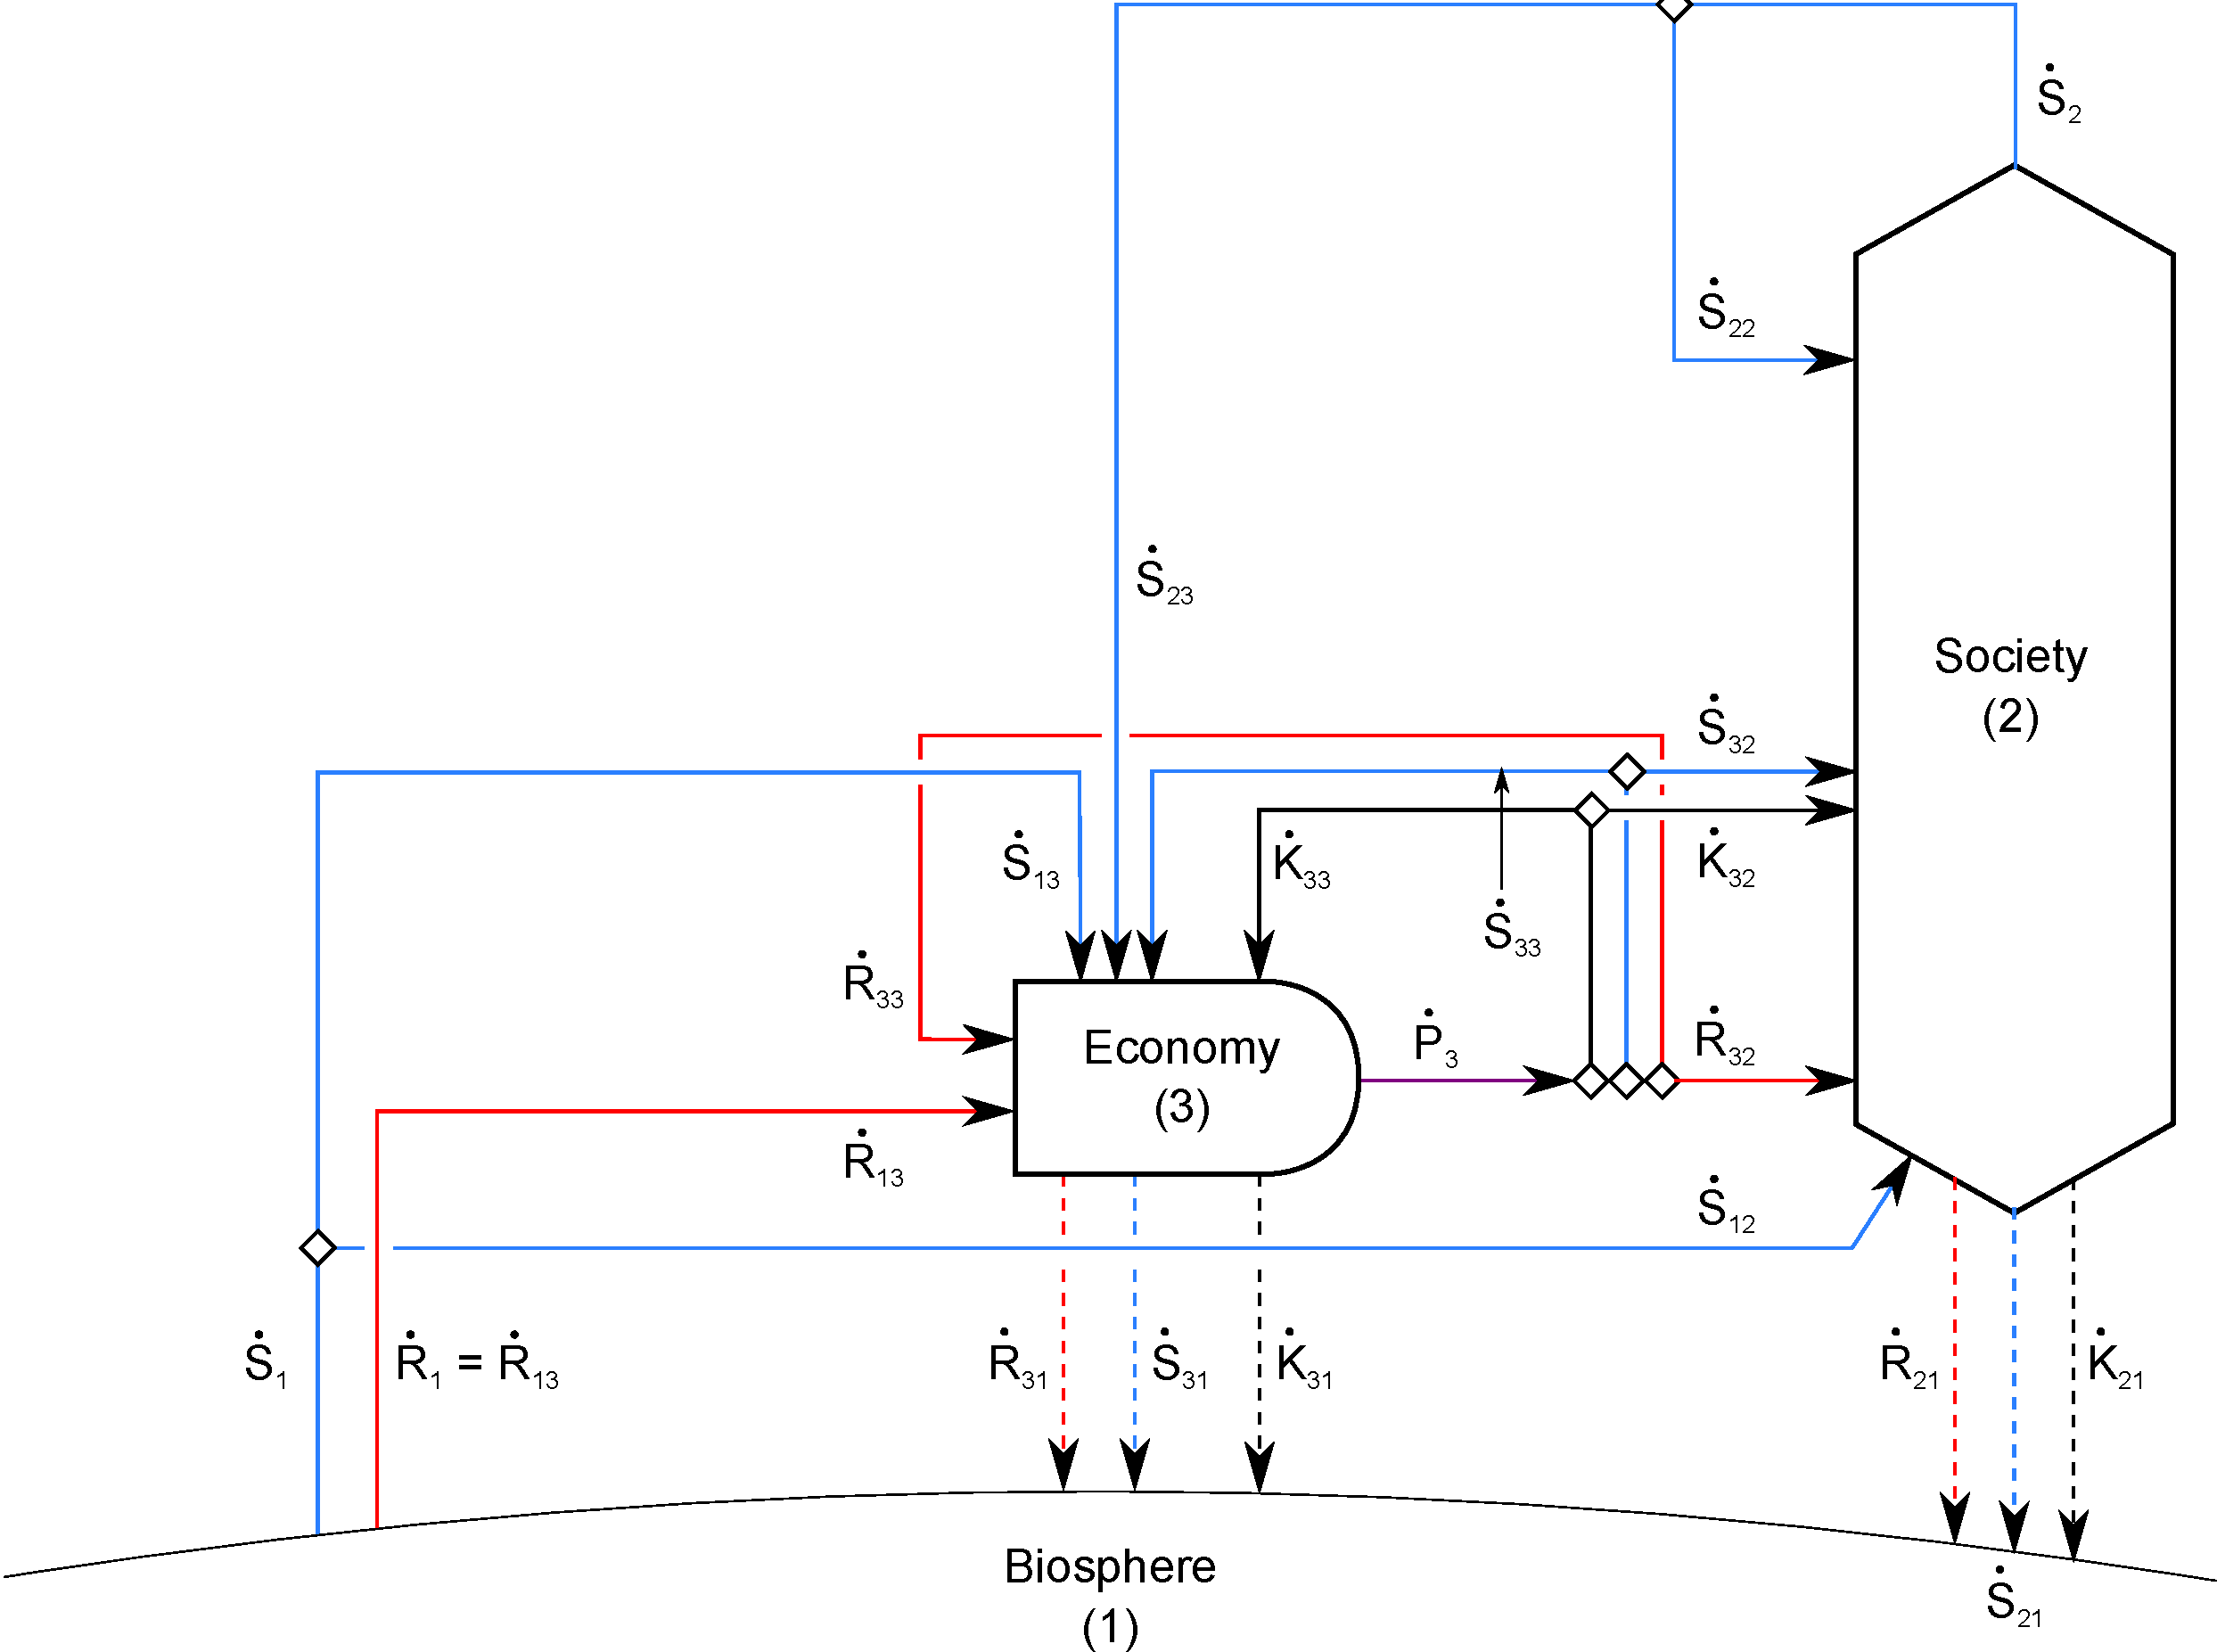
\includegraphics[width=0.8\linewidth]{Part_1/Chapter_Materials/images/2_sector_materials.pdf}
\caption{XXXX}
\label{fig:B_materials}
\end{figure}

%%%%%%%%%% Materials: Example C %%%%%%%%%%
\section{Example C: three sector economy}
\label{sec:C_materials}
%%%%%%%%%%

In example C, we differentiate between two production sectors, one produces energy and one produces other goods and services.


\begin{equation} \label{eq:C-CV_R_dot_0a}
	\frac{\mathrm{d}R_{0}}{\mathrm{d}t} 
	+ \frac{\mathrm{d}S_{0}}{\mathrm{d}t}	
	+ \frac{\mathrm{d}K_0}{\mathrm{d}t}
	=  \dot{R}_{10} + \dot{R}_{20} + \dot{R}_{30}
	+ \dot{S}_{10} + \dot{S}_{20} + \dot{S}_{30}
	+ \dot{K}_{10} + \dot{K}_{20} + \dot{K}_{30}
	- \dot{R}_{0} 
	- \dot{S}_{0},
\end{equation}

\begin{equation}
	\dot{R}_{0} = \dot{R}_{02} + \dot{R}_{03}
\end{equation}

\begin{equation}
	\dot{S}_{0} = \dot{S}_{01} + \dot{S}_{02} + \dot{S}_{03}
\end{equation}

 \begin{equation} \label{eq:C-CV_R_dot_0b}
 	\frac{\mathrm{d}R_{0}}{\mathrm{d}t} 
 	+ \frac{\mathrm{d}S_{0}}{\mathrm{d}t}	
 	+ \frac{\mathrm{d}K_0}{\mathrm{d}t}
 	=  \dot{R}_{10} + \dot{R}_{20} + \dot{R}_{30}
 	+ \dot{S}_{10} + \dot{S}_{20} + \dot{S}_{30}
 	+ \dot{K}_{10} + \dot{K}_{20} + \dot{K}_{30}
 	- \dot{R}_{02} - \dot{R}_{03} 
 	- \dot{S}_{01} - \dot{S}_{02} - \dot{S}_{03},
 \end{equation}
 
 \begin{equation} \label{eq:C-CV_R_dot_1}
 	\frac{\mathrm{d}R_{1}}{\mathrm{d}t} 
	+ \frac{\mathrm{d}S_{1}}{\mathrm{d}t}
 	+ \frac{\mathrm{d}K_{1}}{\mathrm{d}t}
 	=  \dot{R}_{21} + \dot{R}_{31}
 	+ \dot{S}_{01} + \dot{S}_{11} 
	+ \dot{S}_{21} + \dot{S}_{31}
 	+ \dot{K}_{21} + \dot{K}_{31}
 	- \dot{S}_{1} 
	- \dot{R}_{10} 
 	- \dot{S}_{10} 
 	- \dot{K}_{10},
 \end{equation}
 
 \begin{equation} \label{eq:C-CV_R_dot_2}
 	\frac{\mathrm{d}R_{2}}{\mathrm{d}t} 
	+ \frac{\mathrm{d}S_{2}}{\mathrm{d}t}
 	+ \frac{\mathrm{d}K_{2}}{\mathrm{d}t}
 	=  \dot{R}_{02} + \dot{R}_{22} + \dot{R}_{32}
 	+ \dot{S}_{02} + \dot{S}_{12} 
	+ \dot{S}_{22} + \dot{S}_{32} 
 	+ \dot{K}_{22} + \dot{K}_{32}
 	- \dot{P}_{2}
 	- \dot{R}_{20} 
 	- \dot{S}_{20} 
 	- \dot{K}_{20},
 \end{equation}
 
 \begin{equation} \label{eq:C-CV_R_dot_3}
 	\frac{\mathrm{d}R_{3}}{\mathrm{d}t} 
	+ \frac{\mathrm{d}S_{3}}{\mathrm{d}t}
 	+ \frac{\mathrm{d}K_{3}}{\mathrm{d}t}
 	=  \dot{R}_{03} + \dot{R}_{23} + \dot{R}_{33}
 	+ \dot{S}_{03} + \dot{S}_{13} 
	+ \dot{S}_{23} + \dot{S}_{33} 
 	+ \dot{K}_{23} + \dot{K}_{33}
 	- \dot{P}_{3}
 	- \dot{R}_{30} 
 	- \dot{S}_{30} 
 	- \dot{K}_{30},
 \end{equation}

\begin{equation}\label{eq:C-dR_dt_zero}
	\frac{\mathrm{d}R_{1}}{\mathrm{d}t} = \frac{\mathrm{d}R_{2}}{\mathrm{d}t} = \frac{\mathrm{d}R_{3}}{\mathrm{d}t} = 0
\end{equation}

\begin{equation}\label{eq:C-dS_dt_zero}
	\frac{\mathrm{d}S_{1}}{\mathrm{d}t} = \frac{\mathrm{d}S_{2}}{\mathrm{d}t} = \frac{\mathrm{d}S_{3}}{\mathrm{d}t} = 0
\end{equation}

\begin{equation} \label{eq:C-CV_K_dot_2}
	\frac{\mathrm{d}K_{2}}{\mathrm{d}t}
	=  \dot{K}_{22} + \dot{K}_{32} 
	- \dot{K}_{20},
\end{equation}

\begin{equation} \label{eq:C-CV_K_dot_3}
	\frac{\mathrm{d}K_{2}}{\mathrm{d}t}
	=  \dot{K}_{23} + \dot{K}_{33} 
	- \dot{K}_{30},
\end{equation}

 \begin{equation} \label{eq:C-CV_R_dot_1b}
 	\frac{\mathrm{d}K_{1}}{\mathrm{d}t}
 	=  \dot{R}_{21} + \dot{R}_{31}
 	+ \dot{S}_{01} + \dot{S}_{11} 
	+ \dot{S}_{21} + \dot{S}_{31}
 	+ \dot{K}_{21} + \dot{K}_{31}
 	- \dot{S}_{1} 
	- \dot{R}_{10} 
 	- \dot{S}_{10} 
 	- \dot{K}_{10},
 \end{equation}
 
 \begin{equation} \label{eq:C-CV_R_dot_2b}
 	\frac{\mathrm{d}K_{2}}{\mathrm{d}t}
 	=  \dot{R}_{02} + \dot{R}_{22} + \dot{R}_{32}
 	+ \dot{S}_{02} + \dot{S}_{12} 
	+ \dot{S}_{22} + \dot{S}_{32} 
 	+ \dot{K}_{22} + \dot{K}_{32}
 	- \dot{P}_{2}
 	- \dot{R}_{20} 
 	- \dot{S}_{20} 
 	- \dot{K}_{20}
	=  \dot{K}_{22} + \dot{K}_{32} 
	- \dot{K}_{20},
 \end{equation}
 
 \begin{equation} \label{eq:C-CV_R_dot_3}
 	\frac{\mathrm{d}K_{3}}{\mathrm{d}t}
 	=  \dot{R}_{03} + \dot{R}_{23} + \dot{R}_{33}
 	+ \dot{S}_{03} + \dot{S}_{13} 
	+ \dot{S}_{23} + \dot{S}_{33} 
 	+ \dot{K}_{23} + \dot{K}_{33}
 	- \dot{P}_{3}
 	- \dot{R}_{30} 
 	- \dot{S}_{30} 
 	- \dot{K}_{30}
	=  \dot{K}_{23} + \dot{K}_{33} 
	- \dot{K}_{30},
 \end{equation}


\begin{figure}[h!]
\centering
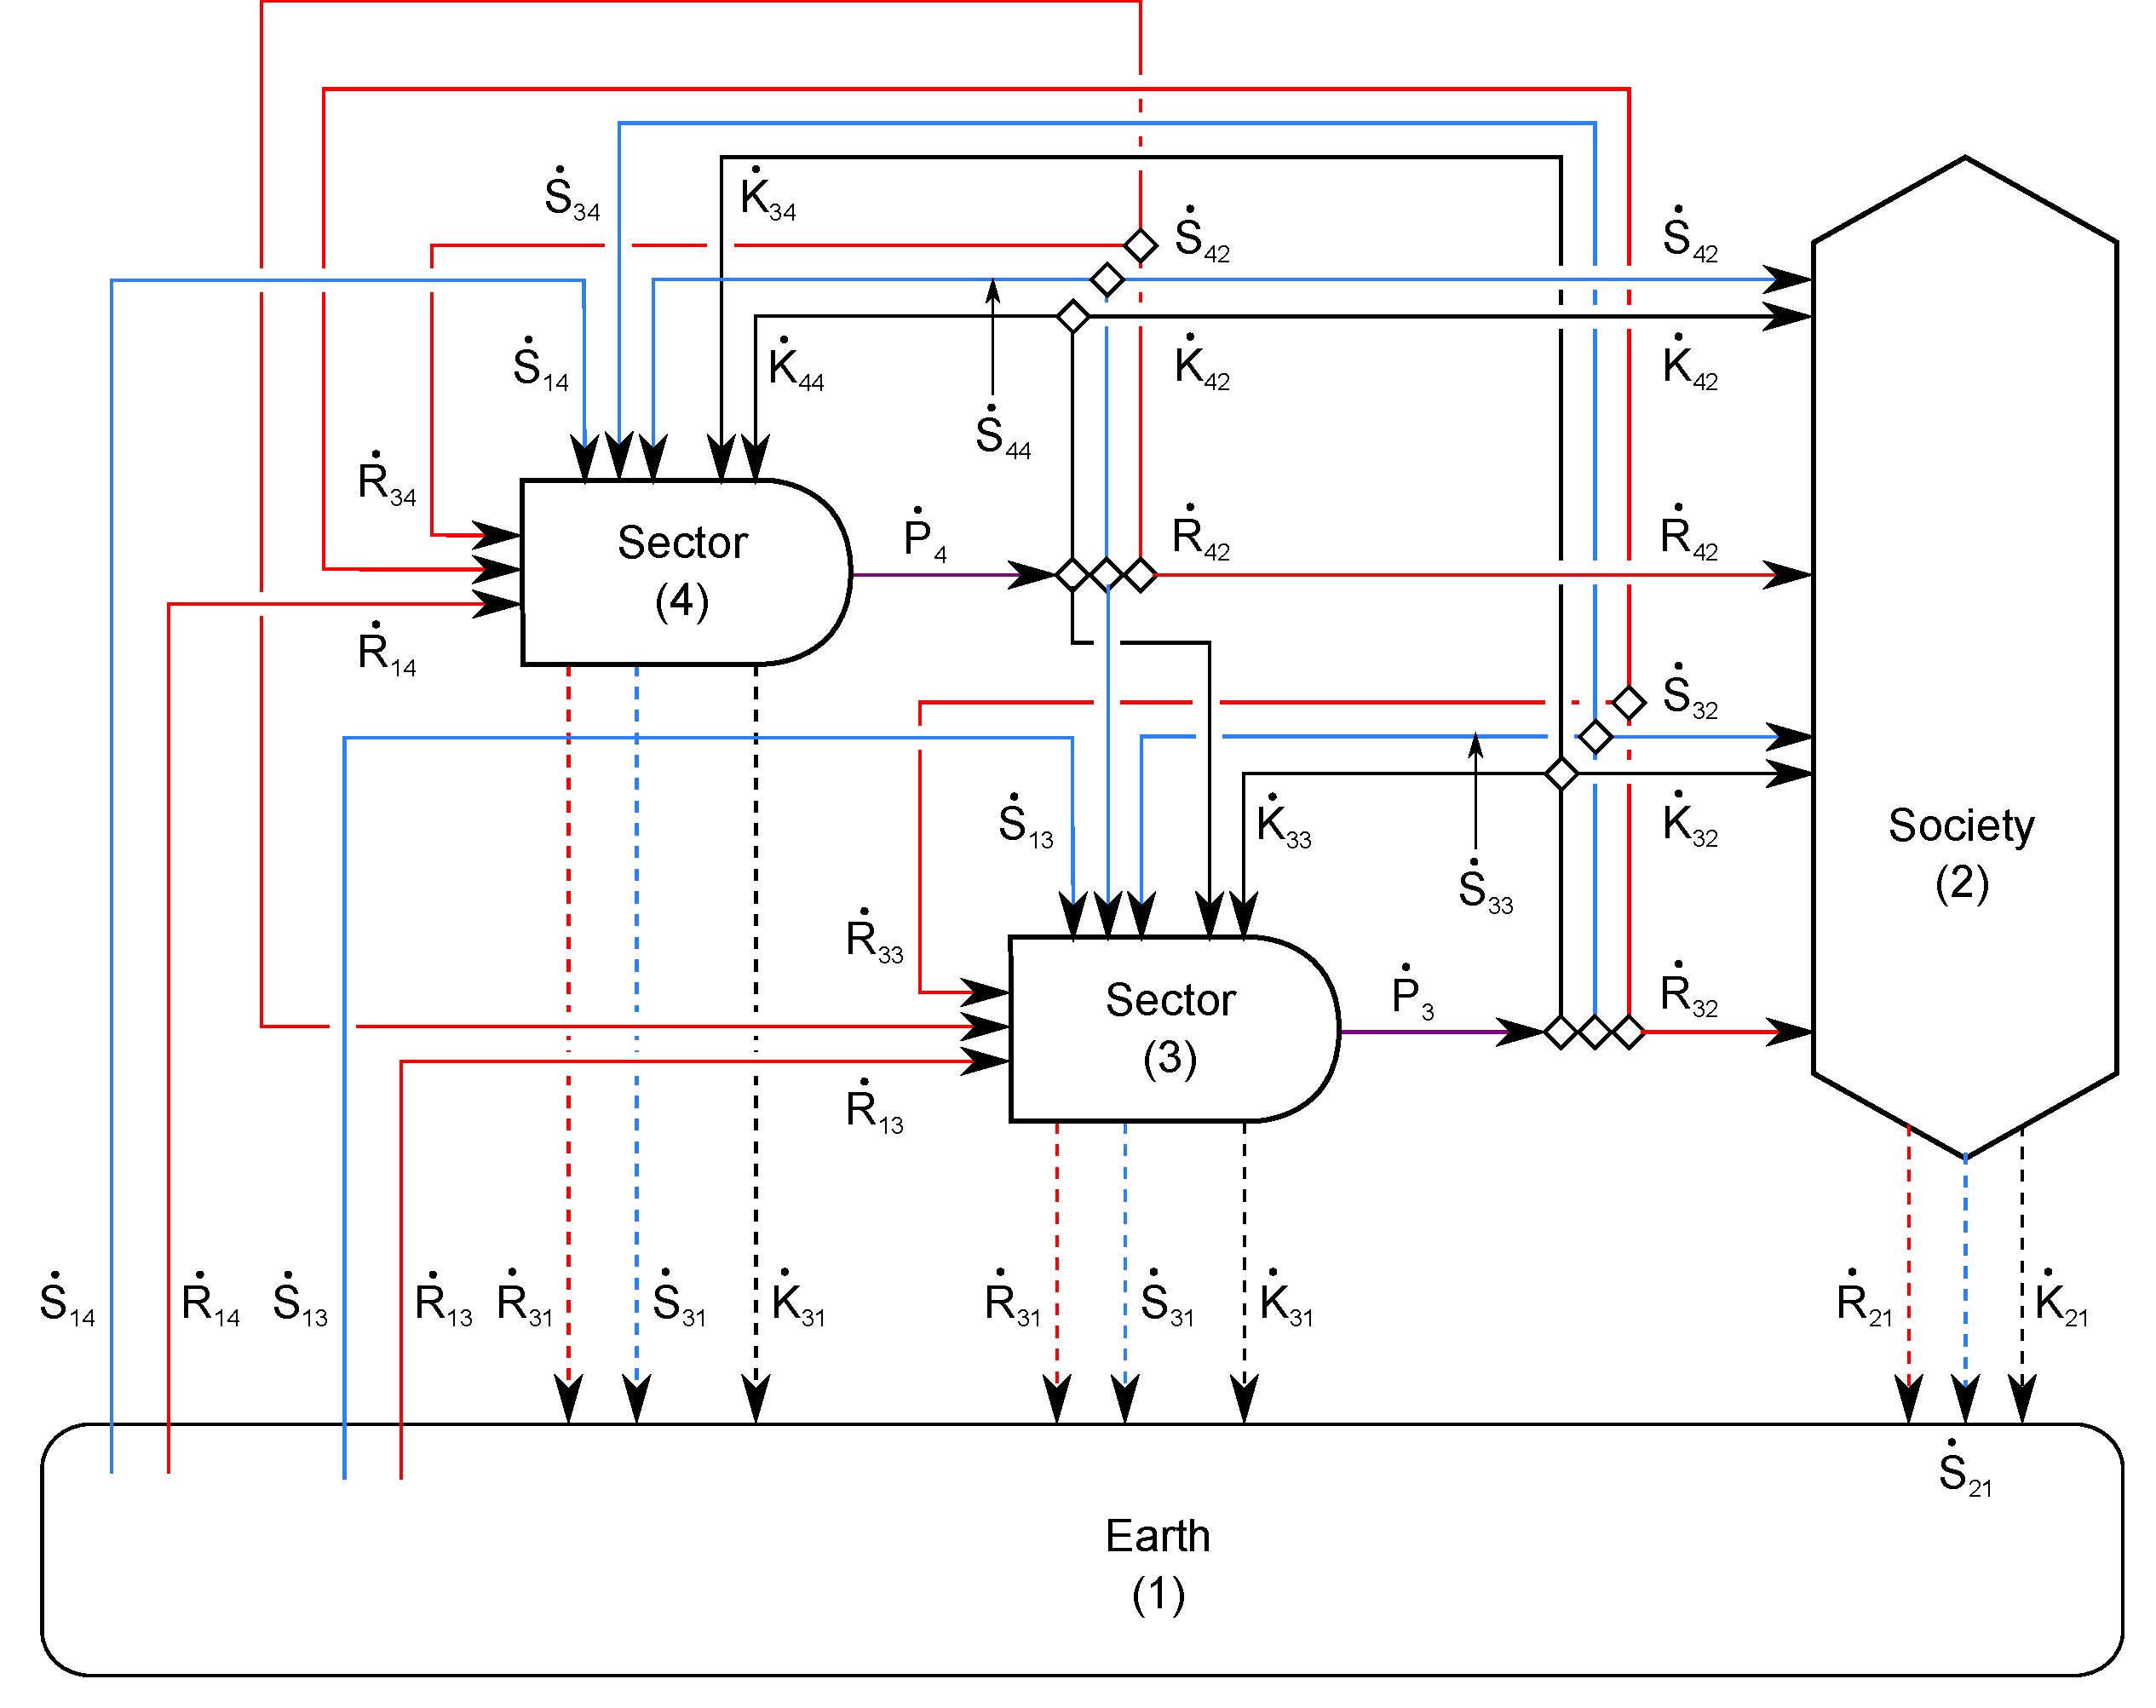
\includegraphics[width=0.8\linewidth]{Part_1/Chapter_Materials/images/3_sector_materials.pdf}
\caption{XXXX}
\label{fig:C_materials}
\end{figure}

\begin{figure}[h!]
\centering
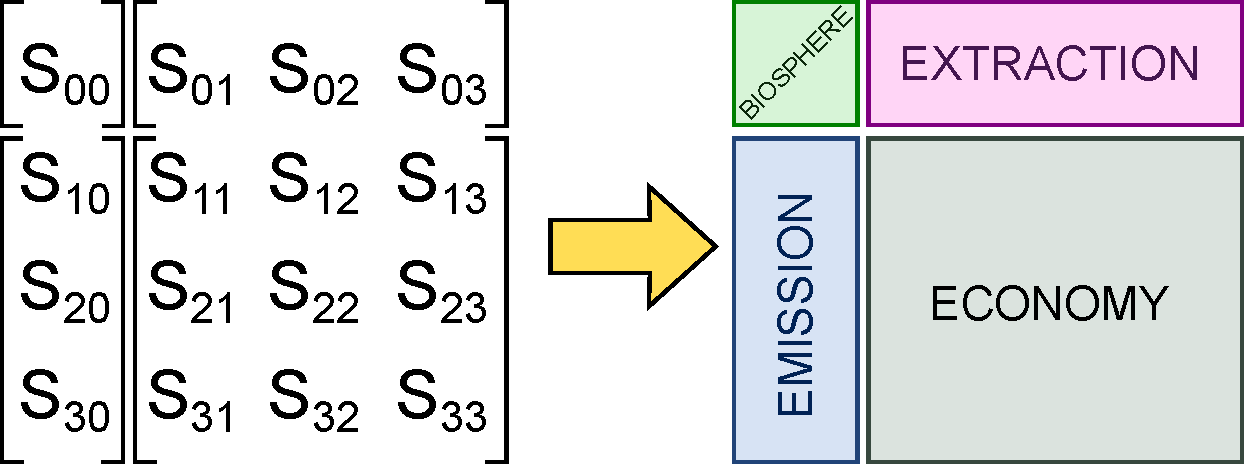
\includegraphics[width=0.8\linewidth]{Part_1/Chapter_Materials/images/Matrix.pdf}
\caption{XXXX}
\label{fig:C_mat_matrix}
\end{figure}

%%%%%%%%%% Materials: Auto industry example %%%%%%%%%%
\section{Materials in the auto industry}
\label{sec:materials_auto}
%%%%%%%%%%

%%%%%%%%%% Materials: Summary %%%%%%%%%%
\section{Summary}
\label{sec:materials_summary}
%%%%%%%%%%

\bibliography{../../EROI_review_v2}
\bibliographystyle{unsrt}


% Always give a unique label
% and use \ref{<label>} for cross-references
% and \cite{<label>} for bibliographic references
% use \sectionmark{}
% to alter or adjust the section heading in the running head
%% Instead of simply listing headings of different levels we recommend to let every heading be followed by at least a short passage of text. Furtheron please use the \LaTeX\ automatism for all your cross-references and citations.

%% Please note that the first line of text that follows a heading is not indented, whereas the first lines of all sequent paragraphs are.

%% Use the standard \verb|equation| environment to typeset your equations, e.g.
%
%% \begin{equation}
%% a \times b = c\;,
%% \end{equation}
%
%% however, for multiline equations we recommend to use the \verb|eqnarray|
%% environment\footnote{In physics texts please activate the class option \texttt{vecphys} to depict your vectors in \textbf{\itshape boldface-italic} type - as is customary for a wide range of physical jects.}.
%% \begin{eqnarray}
%% a \times b = c \nonumber\\
%% \vec{a} \cdot \vec{b}=\vec{c}
%% \label{eq:01}
%% \end{eqnarray}

%% \section{section Heading}
%% \label{sec:2}
%% Instead of simply listing headings of different levels we recommend to let every heading be followed by at least a short passage of text. Furtheron please use the \LaTeX\ automatism for all your cross-references\index{cross-references} and citations\index{citations} as has already been described in Sect.~\ref{sec:2}.

%% \begin{quotation}
%% Please do not use quotation marks when quoting texts! Simply use the \verb|quotation| environment -- it will automatically render Springer's preferred layout.
%% \end{quotation}


%% \section{section Heading}
%% Instead of simply listing headings of different levels we recommend to let every heading be followed by at least a short passage of text. Furtheron please use the \LaTeX\ automatism for all your cross-references and citations as has already been described in Sect.~\ref{sec:2}, see also Fig.~\ref{fig:1}\footnote{If you copy text passages, figures, or tables from other works, you must obtain \textit{permission} from the copyright holder (usually the original publisher). Please enclose the signed permission with the manucript. The sources\index{permission to print} must be acknowledged either in the captions, as footnotes or in a separate section of the book.}

%% Please note that the first line of text that follows a heading is not indented, whereas the first lines of all sequent paragraphs are.

% For figures use
%
%% \begin{figure}[b]
%% \sidecaption
% Use the relevant command for your figure-insertion program
% to insert the figure file.
% For example, with the option graphics use
%% \includegraphics[scale=.65]{figure}
%
% If not, use
%\picplace{5cm}{2cm} % Give the correct figure height and width in cm
%
%% \caption{If the width of the figure is less than 7.8 cm use the \texttt{sidecapion} command to flush the caption on the left side of the page. If the figure is positioned at the top of the page, align the sidecaption with the top of the figure -- to achieve this you simply need to use the optional argument \texttt{[t]} with the \texttt{sidecaption} command}
%% \label{fig:1}       % Give a unique label
%% \end{figure}


%% \paragraph{Paragraph Heading} %
%% Instead of simply listing headings of different levels we recommend to let every heading be followed by at least a short passage of text. Furtheron please use the \LaTeX\ automatism for all your cross-references and citations as has already been described in Sect.~\ref{sec:2}.

%% Please note that the first line of text that follows a heading is not indented, whereas the first lines of all sequent paragraphs are.

%% For typesetting numbered lists we recommend to use the \verb|enumerate| environment -- it will automatically render Springer's preferred layout.

%% \begin{enumerate}
%% \item{Livelihood and survival mobility are oftentimes coutcomes of uneven socioeconomic development.}
%% \begin{enumerate}
%% \item{Livelihood and survival mobility are oftentimes coutcomes of uneven socioeconomic development.}
%% \item{Livelihood and survival mobility are oftentimes coutcomes of uneven socioeconomic development.}
%% \end{enumerate}
%% \item{Livelihood and survival mobility are oftentimes coutcomes of uneven socioeconomic development.}
%% \end{enumerate}


%% \paragraph{paragraph Heading} In order to avoid simply listing headings of different levels we recommend to let every heading be followed by at least a short passage of text. Use the \LaTeX\ automatism for all your cross-references and citations as has already been described in Sect.~\ref{sec:2}, see also Fig.~\ref{fig:2}.

%% Please note that the first line of text that follows a heading is not indented, whereas the first lines of all sequent paragraphs are.

%% For unnumbered list we recommend to use the \verb|itemize| environment -- it will automatically render Springer's preferred layout.

%% \begin{itemize}
%% \item{Livelihood and survival mobility are oftentimes coutcomes of uneven socioeconomic development, cf. Table~\ref{tab:1}.}
%% \begin{itemize}
%% \item{Livelihood and survival mobility are oftentimes coutcomes of uneven socioeconomic development.}
%% \item{Livelihood and survival mobility are oftentimes coutcomes of uneven socioeconomic development.}
%% \end{itemize}
%% \item{Livelihood and survival mobility are oftentimes coutcomes of uneven socioeconomic development.}
%% \end{itemize}

%% \begin{figure}[t]
%% \sidecaption[t]
% Use the relevant command for your figure-insertion program
% to insert the figure file.
% For example, with the option graphics use
%% \includegraphics[scale=.65]{figure}
%
% If not, use
%\picplace{5cm}{2cm} % Give the correct figure height and width in cm
%
%% \caption{Please write your figure caption here}
%% \label{fig:2}       % Give a unique label
%% \end{figure}

%% \runinhead{Run-in Heading Boldface Version} Use the \LaTeX\ automatism for all your cross-references and citations as has already been described in Sect.~\ref{sec:2}.

%% \runinhead{Run-in Heading Italic Version} Use the \LaTeX\ automatism for all your cross-refer\-ences and citations as has already been described in Sect.~\ref{sec:2}\index{paragraph}.
% Use the \index{} command to code your index words
%
% For tables use
%
%% \begin{table}
%% \caption{Please write your table caption here}
%% \label{tab:1}       % Give a unique label
%
% For LaTeX tables use
%
%% \begin{tabular}{p{2cm}p{2.4cm}p{2cm}p{4.9cm}}
%% \hline\noalign{\smallskip}
%% Classes & class & Length & Action Mechanism  \\
%% \noalign{\smallskip}\svhline\noalign{\smallskip}
%% Translation & mRNA$^a$  & 22 (19--25) & Translation repression, mRNA cleavage\\
%% Translation & mRNA cleavage & 21 & mRNA cleavage\\
%% Translation & mRNA  & 21--22 & mRNA cleavage\\
%%Translation & mRNA  & 24--26 & Histone and DNA Modification\\
%%\noalign{\smallskip}\hline\noalign{\smallskip}
%%\end{tabular}
%%$^a$ Table foot note (with superscript)
%%\end{table}
%
%% \section{Section Heading}
%%\label{sec:3}
% Always give a unique label
% and use \ref{<label>} for cross-references
% and \cite{<label>} for bibliographic references
% use \sectionmark{}
% to alter or adjust the section heading in the running head
%% Instead of simply listing headings of different levels we recommend to let every heading be followed by at least a short passage of text. Furtheron please use the \LaTeX\ automatism for all your cross-references and citations as has already been described in Sect.~\ref{sec:2}.

%% Please note that the first line of text that follows a heading is not indented, whereas the first lines of all sequent paragraphs are.

%%If you want to list definitions or the like we recommend to use the Springer-enhanced \verb|description| environment -- it will automatically render Springer's preferred layout.

%%\begin{description}[Type 1]
%%\item[Type 1]{That addresses central themes pertainng to migration, health, and disease. In Sect.~\ref{sec:1}, Wilson discusses the role of human migration in infectious disease distributions and patterns.}
%%\item[Type 2]{That addresses central themes pertainng to migration, health, and disease. In Sect.~\ref{sec:2}, Wilson discusses the role of human migration in infectious disease distributions and patterns.}
%%\end{description}

%%\section{section Heading} %
%% In order to avoid simply listing headings of different levels we recommend to let every heading be followed by at least a short passage of text. Use the \LaTeX\ automatism for all your cross-references and citations citations as has already been described in Sect.~\ref{sec:2}.

%% Please note that the first line of text that follows a heading is not indented, whereas the first lines of all sequent paragraphs are.

%% \begin{svgraybox}
%% If you want to emphasize complete paragraphs of texts we recommend to use the newly defined Springer class option \verb|graybox| and the newly defined environment \verb|svgraybox|. This will produce a 15 percent screened box 'behind' your text.

%% If you want to emphasize complete paragraphs of texts we recommend to use the newly defined Springer class option and environment \verb|svgraybox|. This will produce a 15 percent screened box 'behind' your text.
%% \end{svgraybox}


%% \section{section Heading}
%%Instead of simply listing headings of different levels we recommend to let every heading be followed by at least a short passage of text. Furtheron please use the \LaTeX\ automatism for all your cross-references and citations as has already been described in Sect.~\ref{sec:2}.

%% Please note that the first line of text that follows a heading is not indented, whereas the first lines of all sequent paragraphs are.

%% \begin{theorem}
%% Theorem text goes here.
%% \end{theorem}
%
% or
%
%% \begin{definition}
%% Definition text goes here.
%% \end{definition}

%% \begin{proof}
%\smartqed
%% Proof text goes here.
%% \qed
%% \end{proof}

%%\paragraph{Paragraph Heading} %
%% Instead of simply listing headings of different levels we recommend to let every heading be followed by at least a short passage of text. Furtheron please use the \LaTeX\ automatism for all your cross-references and citations as has already been described in Sect.~\ref{sec:2}.

%% Note that the first line of text that follows a heading is not indented, whereas the first lines of all subsequent paragraphs are.
%
% For built-in environments use
%
%%\begin{theorem}
%%Theorem text goes here.
%%\end{theorem}
%
%%\begin{definition}
%%Definition text goes here.
%%\end{definition}
%
%%\begin{proof}
%%\smartqed
%% Proof text goes here.
%%\qed
%%\end{proof}
%
%% \begin{acknowledgement}
%% If you want to include acknowledgments of assistance and the like at the end of an individual chapter please use the \verb|acknowledgement| environment -- it will automatically render Springer's preferred layout.
%% \end{acknowledgement}
%
%% \section*{Appendix}
%% \addcontentsline{toc}{section}{Appendix}
%
%% When placed at the end of a chapter or contribution (as opposed to at the end of the book), the numbering of tables, figures, and equations in the appendix section continues on from that in the main text. Hence please \textit{do not} use the \verb|appendix| command when writing an appendix at the end of your chapter or contribution. If there is only one the appendix is designated ``Appendix'', or ``Appendix 1'', or ``Appendix 2'', etc. if there is more than one.

%% \begin{equation}
%% a \times b = c
%% \end{equation}
% Problems or Exercises should be sorted chapterwise
%% \section*{Problems}
%% \addcontentsline{toc}{section}{Problems}
%
% Use the following environment.
% Don't forget to label each problem;
% the label is needed for the solutions' environment
%% \begin{prob}
%% \label{prob1}
%% A given problem or Excercise is described here. The
%% problem is described here. The problem is described here.
%% \end{prob}

%% \begin{prob}
%% \label{prob2}
%% \textbf{Problem Heading}\\
%% (a) The first part of the problem is described here.\\
%% (b) The second part of the problem is described here.
%% \end{prob}


